\documentclass[11pt,a4paper]{article}
\usepackage[margin=24mm,headheight=14pt,includeheadfoot]{geometry}
\usepackage{amsmath,amsthm,booktabs,longtable,array}
\usepackage[T1]{fontenc}
\usepackage{newtxtext,newtxmath}
\usepackage{microtype,graphicx,pdflscape,caption,fancyhdr,xcolor}
\usepackage{hyperref}
\definecolor{ink}{HTML}{23384D}
\hypersetup{colorlinks=true,urlcolor=ink,linkcolor=ink,citecolor=ink,
  pdftitle={When conditional variance harms KSIVI on the X-shaped target},
  pdfauthor={StatComp variance investigation}}
\newtheorem{proposition}{Proposition}[section]
\newtheorem{corollary}[proposition]{Corollary}
\numberwithin{equation}{section}
\newcommand{\E}{\mathbb E}
\newcommand{\Var}{\operatorname{Var}}
\newcommand{\Cov}{\operatorname{Cov}}
\newcommand{\tr}{\operatorname{tr}}
\newcommand{\diag}{\operatorname{diag}}
\setlength{\parskip}{4pt}
\setlength{\parindent}{1em}
\setlength{\tabcolsep}{4pt}
\renewcommand{\arraystretch}{1.16}
\setlength{\emergencystretch}{1.5em}
\captionsetup{font=small,labelfont=bf,labelsep=period}
\pagestyle{fancy}
\fancyhf{}
\fancyhead[L]{\small\itshape KSIVI on the X-shaped target}
\fancyhead[R]{\small Variance investigation}
\fancyfoot[C]{\thepage}
\renewcommand{\headrulewidth}{0.3pt}
\title{When conditional variance harms KSIVI on the X-shaped target\\
\large Geometry, representation noise, and optimization boundaries}
\author{Reproducible investigation of the StatComp implementation}
\date{6 October 2026}
\begin{document}
\maketitle
\begin{abstract}
The empirical question is a comparison of training procedures, not a ranking
of variational families. A conditional variance network contains the global
variance model, and the population KSIVI objective depends on the marginal
distribution rather than on its hierarchical representation. The X-shaped
target has an exact representation with a global variance of $0.2I$ and a
mixture of rank-one means. Conditional variance therefore introduces redundant
directions without being necessary for this target. We prove that these
directions can substantially increase conditional-score representation noise
while leaving the marginal distribution unchanged. Independent GPU experiments
separate this mechanism from initialization, kernel bandwidth differentiation,
variance floors, annealing, and target geometry. The evidence supports
representation noise as a major mechanism, amplified by the optimization
schedule, but does not establish a universal inferiority theorem for
conditional variance. All numerical outcomes, including failed explanations
and counterexamples, are retained below.
\end{abstract}

\section{What exactly is the phenomenon?}
Write $\epsilon\sim N(0,I_2)$ and $u\sim N(0,I_2)$ independently. The two
families implemented in this repository are
\[
 x=\mu_\phi(\epsilon)+\sigma_\phi(\epsilon)\odot u,
 \qquad
 x=\mu_\phi(\epsilon)+\sigma_\phi\odot u.
\]
Both means have two width-128 SiLU hidden layers. Conditional variances are
\[
v_j(\epsilon)=\max\{10^{-4},\operatorname{softplus}(a_j(\epsilon))\}.
\]
Global variances have the same softplus transform applied to two learnable
scalars. The conditional model shares its hidden layers between mean and
variance outputs. Changing \texttt{train.vi.var\_lr} does not change its
variance learning rate: the production optimizer creates a separate variance
group only for models with a global \texttt{var\_raw} parameter.

The canonical training policy is Adam $(0.9,0.999)$, initial learning rate
$10^{-3}$, batch size $128$ in each of two independent batches, 50,000 updates,
and StepLR with factor $0.9$ every 1,000 updates. Target scores are multiplied
by $\alpha_t=0.1+0.9\min(t/25000,1)$. The Gaussian kernel and its empirical
median bandwidth are differentiated. The original authors used a global
variance vector in their experiments; their toy architecture and several
optimization choices differ from this repository \cite{cheng,yu}.

The precise empirical comparison is the distribution over random seeds of
the final approximation error under this policy. In the matched experiments,
the initial mean weights are matched, the variance values agree to float32
roundoff, and the training noise streams are paired. A positive difference
\[
 \Delta_s=\mathrm{SW}_2(q^{\rm conditional}_{s,50000},p)
              -\mathrm{SW}_2(q^{\rm global}_{s,50000},p)
\]
means worse conditional performance for seed $s$. The observed paired
differences are: Seed 42: +2.380; Seed 43: +2.480; Seed 44: +0.391. Tables provide additional KL and KSD
diagnostics; a discrepancy in one metric alone is not treated as proof.

This is not a statement that every conditional run fails, that every global
run succeeds, or that conditional variance is inferior under another optimizer,
estimator, architecture, or target. The statistical unit is an independently
trained model, not a sample drawn from it. Three seeds support these concrete
contrasts but do not locate a universal phase transition.

\section{Population objective: the larger family is not intrinsically worse}
Define $s_p=\nabla\log p$, $s_q=\nabla\log q_\phi$, and
$s_c(x,\epsilon)=\nabla_x\log q_\phi(x\mid\epsilon)$. For the Gaussian
conditional layer, $s_c=-u/\sigma_\phi(\epsilon)$. The executable code returns
the \emph{negative} conditional score $u/\sigma$, so its sign is correct.
For an independently fixed kernel,
\[
 L_k(\phi)=\E[k(x,x')f(x,\epsilon)^T f(x',\epsilon')],\qquad
 f=s_p-s_c.
\]
The prime denotes an independent joint draw. Conditional integration gives
the Fisher identity $\E[s_c\mid x]=s_q(x)$, hence
\[
 L_k(\phi)=\E_{q_\phi\otimes q_\phi}
  [k(x,x')(s_p(x)-s_q(x))^T(s_p(x')-s_q(x'))]
 =\operatorname{KSD}_k^2(q_\phi,p).
\]
This is the population identity underlying KSIVI \cite{cheng}. It remains
valid for a heteroscedastic conditional layer under the usual integrability
and differentiation conditions. There is no additional population Fisher
penalty for conditional variance and no inevitable population bias caused by
conditioning the variance. The conditional network can realize the global
network by setting its variance-output weights to zero and choosing constant
biases. Therefore
\[
 \inf_{\phi\in\Phi_{\rm conditional}}L_k(\phi)
 \ \leq\ \inf_{\phi\in\Phi_{\rm global}}L_k(\phi).
\]
This inequality concerns global optimization of a fixed population objective;
it says nothing about the outcome of finite stochastic Adam training.

For annealed scores the same calculation yields the KSD against
$p_\alpha(x)=p(x)^\alpha/Z_\alpha$. Here $\alpha\geq0.1$, so the target is
proper. It is a moving objective until update 25,000, not simply noisy training
on $p$ throughout. In particular $p^\alpha$ is generally not the mixture of
the individually tempered Gaussian components.

\section{Exact target geometry and a representational boundary}
The target is
\[
 p=\tfrac12N(0,\Sigma_+)+\tfrac12N(0,\Sigma_-),\quad
 \Sigma_\pm=\begin{pmatrix}2&\pm1.8\\\pm1.8&2\end{pmatrix}.
\]
Its eigenvalues are $3.8$ and $0.2$. Let $S\in\{-1,+1\}$ be equiprobable,
let $T\sim N(0,1)$ and $U\sim N(0,I_2)$ independently. Then
\begin{equation}
 X=\sqrt{1.8}\,T(1,S)^T+\sqrt{0.2}\,U
 \label{eq:exact}
\end{equation}
has exactly density $p$. Conditional on $S$, the covariance is $\Sigma_S$.
The global Gaussian layer supplies the narrow transverse width, while the
mixing means supply the long arms. This is a distributional construction;
a finite continuous neural mean approximates the discrete branch switch.
It is not a claim that a finite width-128 network represents the switch exactly.

\begin{proposition}[Exact global-noise boundary]
For an unrestricted mixing distribution of means and independent Gaussian
noise $N(0,D)$ with $D=\diag(d_1,d_2)\succeq0$, an exact representation of
$p$ exists if and only if $\Sigma_\pm-D\succeq0$. Equivalently,
\[
 d_1\leq2,\quad d_2\leq2,\quad (2-d_1)(2-d_2)\geq3.24.
\]
For isotropic noise $D=vI$, this is $0\leq v\leq0.2$.
\end{proposition}
\begin{proof}
Sufficiency follows by mixing $N(0,\Sigma_+-D)$ and
$N(0,\Sigma_--D)$ and adding $N(0,D)$. Degenerate Gaussian mean
components are allowed. For necessity, suppose a direction $w$ satisfies
$w^TDw>\min_s w^T\Sigma_s w$. The characteristic function of the mixing
mean in this direction would be
\[
 \tfrac12\sum_{s\in\{+,-\}}
  \exp\{-t^2w^T(\Sigma_s-D)w/2\}.
\]
At least one term grows without bound as $|t|\to\infty$, contradicting the
bound $|\varphi(t)|\leq1$ for a characteristic function. The matrix and
diagonal conditions follow.
\end{proof}
Conditional variance offers no needed expressiveness for this target in the
closure of flexible mean mixtures. The upper endpoint $0.2$ also gives a
useful interpretation to successful learned global variances near $0.2$;
their proximity to that value is not, by itself, a proof of exact recovery.
For the correlation-controlled target with off-diagonals $\pm2\rho$,
the corresponding isotropic boundary is $2(1-|\rho|)$: $2$, $1$, and $0.2$
at $\rho=0$, $0.5$, and $0.9$. Sharper arms require smaller component noise.

For diagnostics, $\E X=0$, $\Cov X=2I$, and $\E\|X\|^4=44.96$.
With rotated coordinates $A=(X_1+X_2)/\sqrt2$ and
$B=(X_1-X_2)/\sqrt2$, $\E A^2B^2=3.8\times0.2=0.76$.
An isotropic $N(0,2I)$ has the same covariance but cross-fourth moment $4$.
Covariance recovery alone therefore cannot validate the X-shaped geometry.

\section{Why conditional scores can become noisy without changing the marginal}
\begin{proposition}[Residual representation noise]
Assume $q_\phi=p$, Gaussian conditionals with diagonal covariance
$D(\epsilon)$, and finite second moments of the conditional score. Then
\begin{equation}
 \E\|s_p(X)-s_c(X,\epsilon)\|^2
 =\E\tr D(\epsilon)^{-1}-\E_p\|s_p(X)\|^2.
 \label{eq:noise}
\end{equation}
\end{proposition}
\begin{proof}
Given $X$, the mean conditional score equals $s_p(X)$. Expanding the
squared residual and using that identity reduces the expression to
$\E\|s_c\|^2-\E\|s_p\|^2$. Given $\epsilon$, the Gaussian score has
second moment $\tr D(\epsilon)^{-1}$.
\end{proof}
At the marginal optimum, $f$ has conditional mean zero but need not itself
be zero. For Gaussian kernels $k(x,x)=1$, the RKHS random feature
$Y=k(X,\cdot)\otimes f$ has zero mean and covariance operator $C$ with
$\tr C$ equal to the right side of (\ref{eq:noise}). Two independent
size-$N$ averages give the loss estimate $\langle\bar Y,\bar Y'\rangle$,
whose variance at this optimum is $\tr(C^2)/N^2$. Away from the optimum,
if $m=\E Y$, the variance is
\[
 \frac{2}{N}\langle m,Cm\rangle+\frac{1}{N^2}\tr(C^2).
\]
These are loss-variance identities, not a substitute for a gradient-variance
bound. Increasing $\tr C$ does not establish a monotone increase in every
direction of $C$ or in every gradient coordinate.

For each variance coordinate, Jensen gives
$\E[1/v_j]\geq1/\E[v_j]$, strictly if $v_j$ is nonconstant.
A moderate \emph{mean} variance can thus conceal a large representation
noise budget when a small subset of latent inputs approaches the floor.
At $v=10^{-4}$ the component score standard deviation is $100$, compared
with approximately $2.24$ at $v=0.2$. These scales do not automatically
establish a gradient failure, because target and conditional score terms
can cancel. We measure gradients separately.

For $\ell_j=\log\sigma_j$ and fixed mean, the pathwise residual derivative is
\[
 \frac{\partial f_i}{\partial\ell_j}
 =\alpha\,H_{p,ij}(X)\sigma_j u_j
          -\mathbb 1\{i=j\}\frac{u_j}{\sigma_j}.
\]
Network parameter derivatives multiply these terms by latent-dependent
Jacobians. A conditional variance head supplies many such directions and
shares the trunk with the mean head. Global variance restricts them to two
coordinates and pools updates over all latent inputs. Small variances,
large target curvature, and shared Jacobians can therefore interact.
This is a mechanism, not a theorem that adding parameters always increases
gradient variance under Adam.

\subsection{A counterfactual with exactly equal marginal distributions}
For any $v\in(0,0.2]$, take the mixing means from
$\tfrac12N(0,\Sigma_+-vI)+\tfrac12N(0,\Sigma_--vI)$.
Adding $N(0,vI)$ gives exactly $p$. One may also randomize $v$ between
$0.02$ and $0.2$, since the conditional-on-$v$ marginal is $p$ in both cases.
The random variance has mean $0.11$, exactly matching a constant-$0.11$
representation. This isolates hierarchy and estimator noise from all
approximation error and training path differences. This distributional
simulation is not a finite neural-network representation; the training
experiments provide the architecture-specific link.

The experiment differentiates a common global dilation
$X_\theta=e^\theta X$, $\sigma_\theta=e^\theta\sigma$ at $\theta=0$,
with fixed $h=0.75$. It uses 256 independent repetitions of two size-128
batches. The population loss and its first derivative are zero in every
row. The numerical variances are:
\begin{center}
\begin{tabular}{lrrr}\toprule
Component variance & \shortstack{Conditional\\gradient variance} & \shortstack{Stein\\gradient variance} & $\E\|f\|^2$\\\midrule
0.2 & 0.00253 & 0.00196 & 5.93 \\
0.11 & 0.01002 & 0.00201 & 14.11 \\
0.05 & 0.04286 & 0.00204 & 35.93 \\
0.02 & 0.28042 & 0.00217 & 95.93 \\
0.02/0.20 mixture & 0.07267 & 0.00186 & 50.93 \\
0.002 & 24.45727 & 0.00203 & 995.93 \\
\bottomrule\end{tabular}
\end{center}
The constant-$0.02$ representation has about 110 times the directional
conditional-gradient variance of the constant-$0.2$ representation. The
heteroscedastic representation has about seven times that of its
constant-$0.11$ comparator. The Stein-estimator variance is approximately
$0.002$ across these representations. These measured ratios are finite
Monte Carlo estimates, not universal exponents or constants.

\subsection{An analytic gradient-variance asymptotic, with no fitted coefficient}
\begin{proposition}[Marginal-preserving gradient-noise explosion]
In the constant-$v$ construction above, for fixed $N$ and fixed Gaussian
bandwidth $h>0$, let $g_v$ be the conditional-score estimator's derivative
under global dilation at zero. Then
\[
 \lim_{v\downarrow0}v^2\Var(g_v)
 =\frac{2}{N^2}\E_{X,X'\sim p}
   \left[k_h(X,X')^2\left(2+\frac{\|X-X'\|^2}{h^2}\right)^2\right]>0.
\]
In contrast, the Stein-estimator dilation gradient has exactly the same
distribution for every $v$ in this construction, including the heterogeneous
representation.
\end{proposition}
\begin{proof}
Write $X_i=M_{v,i}+\sqrt v\,U_i$ and $X'_j=M'_{v,j}+\sqrt v\,U'_j$,
where $M_v$ has the residual Gaussian-mixture law and $U,U'$ are standard
two-dimensional normals independent of the means. At zero dilation,
$\partial_\theta k_h=-\|X-X'\|^2k_h/h^2$ and
$\partial_\theta f=H_p(X)X-U/\sqrt v$. The leading pair-gradient term is
\[
 -\frac1v k_h(X,X')\left(2+\frac{\|X-X'\|^2}{h^2}\right)U^TU'.
\]
Couple $M_v$ using the same mixture label and Gaussian coordinates as
$v\downarrow0$, so $M_v\to M_0$ with $M_0\sim p$. The target score and its
derivatives have polynomial growth and these Gaussian mixtures have all
polynomial moments. Consequently $v g_v$ converges in $L^2$ to the average
of these leading terms with $X,X'$ replaced by $M_0,M'_0$. Terms involving
one conditional score vanish after multiplication by $v$. Distinct pair
summands have zero covariance even if they share one index, since the
other centered Gaussian noise has conditional mean zero. Also
$\E(U^TU')^2=2$. This gives the stated positive limit. Finally, the Stein
dilation gradient is a deterministic function of $X,X'$, whose independent
marginal laws are $p$ for every representation. Its entire distribution is
therefore representation invariant.
\end{proof}
The constant can be evaluated by a Gaussian quadratic-form Laplace transform.
The difference $X-X'$ is a half-half mixture of normals with covariance
eigenvalues $(7.6,0.4)$ and $(4,4)$. For either covariance $C$, put
$t=h^{-2}$, $M=\det(I+2tC)^{-1/2}$,
$A=\tr[C(I+2tC)^{-1}]$, and
$B=\tr[(C(I+2tC)^{-1})^2]$. The expectation in the limit is the mixture
average of
\[
 M\{4+4tA+t^2(A^2+2B)\}.
\]
At $h=0.75$, $N=128$, the resulting asymptotic variance is
$9.9824\times10^{-5}/v^2$. It predicts $0.2496$ at $v=0.02$, compared with
the measured $0.2804$; no coefficient was fitted to that measurement. This
is a small-$v$ asymptotic, not an assertion of equality at finite $v$. It
proves a concrete way that small conditional variances can defeat a
uniform gradient-noise guarantee even at an exact marginal optimum.
The actual code has a positive $10^{-4}$ variance floor. The asymptotic
therefore explains potentially very large finite variance constants; it does
not assert that the actual finite-floor runs have infinite variance.

\begin{corollary}[Noise can also contaminate mean updates]
If the same construction dilates only the means,
$X_\theta=e^\theta M_v+\sqrt v\,U$, while holding variance fixed, the
conditional-score gradient still has inverse-square variance growth:
\[
 \lim_{v\downarrow0}v^2\Var(g^{\rm mean}_v)
 =\frac{2}{N^2}\E_{p\otimes p}
   \left[k_h(X,X')^2\frac{\|X-X'\|^4}{h^4}\right]>0.
\]
The Stein-estimator mean-direction gradient has bounded second moment as
$v\downarrow0$ for this target.
\end{corollary}
\begin{proof}
The conditional score no longer differentiates directly, but the kernel
derivative multiplying the two conditional scores has leading term
$-k_h(M_0,M'_0)\|M_0-M'_0\|^2U^TU'/(h^2v)$. The preceding $L^2$
and pair-covariance argument applies. The Stein derivative contains no
inverse variance and is bounded in $L^2$ by polynomial Gaussian moments.
\end{proof}
Dilating mean outputs is an available parameter direction: scale the mean
rows and biases of the final linear layer, leaving the variance rows
unchanged. Thus the mechanism is not confined to the variance-head gradient
under the independently fixed bandwidth of this corollary. Detaching the
entire kernel removes this leading mean-gradient term but changes the update
away from the full KSD gradient; detaching only the bandwidth does not remove
it. Full adaptive-median differentiation needs a separate calculation:
uniform dilation of all points also dilates the median bandwidth, so that
the Gaussian kernel itself is invariant. The fixed-bandwidth coefficient
must not be applied to that adaptive, isotropic mean direction.

This cancellation is not generic across mean parameters. To see why, scale
only the first mean output, an available final-layer row direction. In the
$v\downarrow0$ construction, put $\delta_{ij}=M_{0,i}-M'_{0,j}$,
$D_{ij}=\|\delta_{ij}\|^2$. Let $(a,b)$ be the unique median-distance pair
and $r_* = \delta_{ab,1}^2/D_{ab}$. For the implemented median rule,
$h^2=D_{ab}/[2\log(N+1)]$, and differentiating the kernel gives
\[
 \partial_\theta k_{ij}
 =-\frac{k_{ij}}{h^2}(\delta_{ij,1}^2-D_{ij}r_*)=-A_{ij}.
\]
The leading conditional-score pair-average gradient is therefore
$-(N^2v)^{-1}\sum_{ij}A_{ij}U_i^TU'_j$. Conditional on the means, its
variance is $2(N^4v^2)^{-1}\sum_{ij}A_{ij}^2$. The median pair has zero
coefficient, but other pairs do not all have its directional ratio almost
surely for this continuous two-dimensional target and $N=128$. Thus adaptive
bandwidth differentiation does not remove all inverse-variance mean-gradient
terms. This leading-term calculation is distinct from the proved full
fixed-bandwidth variance asymptotic above, and is not a universal bound on
every network-gradient coordinate.

The experiment's reported residual second moments use the exact identity
(\ref{eq:noise}) with the target Fisher information estimated independently
from 200,000 exact target draws. They should not be confused with the
closed-form gradient-asymptotic coefficient, which requires no such estimate.

\section{Equivalent population objective, alternative estimator}
Conditional integration by parts yields the conventional Stein integrand
\[
 h_p(x,y)=k\,s_p(x)^Ts_p(y)+s_p(x)^T\nabla_yk
         +s_p(y)^T\nabla_xk+\tr(\nabla_x\nabla_yk).
\]
For $k=\exp(-\|x-y\|^2/(2h^2))$ this is
\[
 k\left[s_p(x)^Ts_p(y)+
 \frac{(s_p(x)-s_p(y))^T(x-y)}{h^2}
 +\frac{2}{h^2}-\frac{\|x-y\|^2}{h^4}\right].
\]
It removes the explicit $u/\sigma$ term while retaining the same fixed-kernel
population KSD. It still differentiates the sampling map and requires target
score derivatives. It is not claimed to be a universally optimal
Rao--Blackwell estimator. The exact Rao--Blackwell random feature would
replace $s_c$ by $\E[s_c\mid X]=s_q(X)$, which is generally intractable;
the law of total covariance explains why removing latent-label noise is
attractive, but does not rank all integration-by-parts gradient estimators.

In the training comparison, both the Stein variant and the bandwidth-only
control detach the median bandwidth, while retaining spatial kernel
gradients. Their comparison separates the estimator change from bandwidth
detachment. A batch-dependent bandwidth means neither finite-batch loss is
automatically an unbiased estimate of a single fixed-bandwidth population
KSD. In particular, integration by parts for a jointly data-dependent
bandwidth would contain additional derivative terms. The equal-objective
claim is deliberately restricted to independently fixed bandwidths. All
held-out KSD and exact-marginal mechanism experiments obey that restriction.
The additional fixed-$h=0.75$ conditional-versus-Stein training contrast
also removes the adaptive-bandwidth confound; it keeps the same conditional
architecture, target schedule, initialization, and optimizer.

\section{Empirical evidence and the boundaries actually tested}
\subsection{Three-seed, 50,000-update comparisons}
Means (sample standard deviations across trained seeds) are reported below.
Each comparison starts at variance $\operatorname{softplus}(1)=1.31326$.
Mean-network weights and biases are copied from the same seeded global
initialization. Diagnostic sampling restores CPU and CUDA RNG states. The
fast update has a locally verified gradient equal to the production update.
\begin{center}\small
\begin{tabular}{p{6.1cm}rrrr}\toprule
Procedure & $n$ & SW$_2$ & KL$(p\|q)$ & KSD$^2_{h=0.75}$\\\midrule
Conditional: canonical & 3 & $1.965\;(1.136)$ & $1.161\;(0.378)$ & $0.0449\;(0.0307)$ \\
Global: canonical & 3 & $0.214\;(0.130)$ & $0.275\;(0.233)$ & $0.0025\;(0.0018)$ \\
Conditional: Stein estimator & 3 & $0.283\;(0.172)$ & $0.357\;(0.298)$ & $0.0038\;(0.0011)$ \\
Global: Stein estimator & 3 & $0.371\;(0.018)$ & $0.874\;(0.182)$ & $0.0039\;(0.0009)$ \\
Conditional: variance floor 0.2 & 3 & $0.400\;(0.024)$ & $0.579\;(0.029)$ & $0.0057\;(0.0015)$ \\
Conditional: no anneal, constant LR & 3 & $1.276\;(1.486)$ & $0.600\;(0.596)$ & $0.0528\;(0.0770)$ \\
Global: no anneal, constant LR & 3 & $0.167\;(0.022)$ & $0.049\;(0.022)$ & $0.0013\;(0.0008)$ \\
Conditional: detach bandwidth & 3 & $1.360\;(1.050)$ & $1.004\;(0.420)$ & $0.0193\;(0.0115)$ \\
Conditional: fixed h=0.75 & 3 & $0.589\;(0.168)$ & $0.693\;(0.277)$ & $0.0061\;(0.0016)$ \\
Conditional: fixed h, Stein & 3 & $0.565\;(0.188)$ & $0.684\;(0.220)$ & $0.0104\;(0.0067)$ \\
\bottomrule\end{tabular}
\end{center}
The canonical gap appears in all three paired seeds: mean SW$_2$ is 1.965 versus 0.214, and mean forward KL is 1.161 versus 0.275. Raising the conditional variance floor to $0.2$ improves each canonical conditional seed, with mean SW$_2$ 0.400. The adaptive-bandwidth Stein conditional variant also improves each canonical conditional seed, with mean SW$_2$ 0.283; bandwidth detachment alone leaves mean SW$_2$ 1.360.

The fixed-bandwidth comparison sets an important boundary: with $h=0.75$,
Stein improves SW$_2$ for seeds 42 and 43 but worsens it for seed 44.
Its mean forward KL is nearly unchanged and mean held-out KSD is worse.
The adaptive-bandwidth estimator improvement therefore does not establish
a universal benefit from changing estimators, even when the population
objectives agree. A successful Stein conditional run also retains a large
inverse-variance tail: small component variance does not itself imply poor
marginal approximation. It makes the conditional-score estimator noisy;
the optimizer and kernel policy determine how that noise affects learning.

The variance-floor intervention restricts every conditional variance to at
least $0.2$, so the exact construction (\ref{eq:exact}) remains available in
the flexible-mean closure. It also changes optimization geometry and creates
zero gradients through clamped variance outputs. It is therefore a useful
intervention but not a pure measurement of stochastic noise.

The no-annealing, constant-learning-rate comparison changes both the target
path and adaptation budget. It tests a boundary of the observed phenomenon;
it does not identify which of the two changes is responsible. The separate
one-factor screening controls are retained in the appendix.

\subsection{Historical canonical runs and initialization controls}
We audited 334 saved checkpoints. One historical canonical
result per family, seed, and initialization is retained in the table below;
repeated runs using the same seed are not treated as independent seeds.
These are historical comparisons, not matched-mean randomizations: changing
the output layer shape can change initial mean biases under the same seed.
\begin{center}\small
\begin{tabular}{llrrrr}\toprule
Family & Variance initialization & Seed & SW$_2$ & KL$(p\|q)$ & $\E[1/v]$\\\midrule
Global & Default & 44 & 0.138 & 0.085 & 5.0 \\
Global & Default & 45 & 0.118 & 0.084 & 5.0 \\
Global & Default & 46 & 0.128 & 0.033 & 5.0 \\
Conditional & Matched variance & 42 & 0.518 & 0.463 & 29.4 \\
Conditional & Matched variance & 43 & 1.765 & 1.296 & 189.3 \\
Conditional & Matched variance & 44 & 0.705 & 0.962 & 8.2 \\
Conditional & Default & 42 & 4.215 & 1.366 & 2392.7 \\
Conditional & Default & 43 & 1.444 & 0.991 & 628.8 \\
Conditional & Default & 44 & 0.385 & 0.432 & 13.9 \\
Global & Default & 43 & 0.318 & 0.643 & 5.1 \\
Conditional & Default & 45 & 1.632 & 1.178 & 623.7 \\
Conditional & Default & 46 & 0.447 & 0.609 & 10.4 \\
\bottomrule\end{tabular}
\end{center}
Matching only the initial variance in the historical conditional model does
not guarantee recovery. The newer paired comparisons also match the mean
function, which addresses this remaining initialization confound.

\subsection{Broad screening and counterexamples}
The screening study varies batch size, variance floors, network sharing,
annealing duration, learning-rate decay, kernel bandwidth differentiation,
estimator, and target correlation. These are 10,000-update, seed-42 results.
Annealed runs still have $\alpha=0.46$ unless a shorter warmup is specified;
they are measured against the final target for consistency, so their absolute
errors are not final-target convergence claims. At this horizon an unannealed
conditional run beats its global counterpart, and the isotropic Gaussian
control shows no comparable conditional disadvantage. Shared-trunk removal,
larger batches, or bandwidth detachment alone do not establish a complete
explanation of the original failure.

\section{The schedule amplifies sensitivity; the published theorem has limits here}
The canonical scheduler gives learning rate $10^{-3}0.9^{25}\approx
7.18\times10^{-5}$ when the final target first appears. Summing nominal
learning rates gives approximately $9.282$ before that point and $0.666$
after it, through update 50,000. Only about $6.7\%$ of the total nominal
step-size mass is spent on the final target. This is not an upper bound on
Adam displacement, because adaptive normalization matters. It explains why
more late iterations under the same decay need not repair an earlier basin.

Annealing initially favors a broader density; in the arms, transverse Gaussian
variance scales approximately as $0.2/\alpha$. Both families undergo an early
expansion, but latent-specific variance heads can develop different scales,
small-variance tails, and branch imbalance during subsequent contraction.
The temporal diagnostics support this interaction. Neither removing
annealing alone nor changing decay alone is assumed to be a universal cure.

For the present target put $a=2/0.76$ and $b=1.8/0.76$. Up to a constant,
\[
 \log p(x,y)=-\tfrac a2(x^2+y^2)+\log\cosh(bxy),
 \quad s_p=(-ax+by\tanh(bxy),-ay+bx\tanh(bxy)).
\]
In particular,
\[
 \partial_{xx}\log p(0,R)=-a+b^2R^2\longrightarrow\infty.
\]
Thus the global bounded-Hessian assumption used by the KSIVI optimization
theorem is not literally satisfied even by this original toy target. Third
derivatives are likewise unbounded along $x=c/(bR),y=R$ with nonzero fixed
$c$. A local or high-probability truncated analysis may be useful, but it is
not the global theorem as stated. This fact applies to both families and is
not itself a causal explanation of their ordering.

The published convergence result is to an approximate stationary point under
smoothness, variance, and step-size assumptions, not to the global minimizer
or a small KL approximation. Its variance constant also depends on
parameterization smoothness and moments \cite{cheng,yu}. Consequently the
observed outcomes do not contradict an expressiveness or convergence claim
made by that theorem. Spurious minima in KSD descent are an established
possibility \cite{korba}; we do not use a higher-dimensional RBF
non-convergence result as a proof of this two-dimensional failure.

\section{What is established, and what remains an inference?}
\textbf{Established analytically:} population representation invariance;
nested variational families; the exact global Gaussian-noise boundary;
the inverse-variance identity for representation noise; inverse-square
gradient-variance growth in a marginal-preserving counterfactual, including
an available mean-parameter direction; and unbounded target curvature.

\textbf{Established empirically in these experiments:} the numerical seed
comparisons and intervention outcomes in the tables; the gradient-noise
increase at exactly equal marginals; and the independent held-out accuracy
and fixed-bandwidth KSD measurements. Each trained-model directional gradient
comparison uses a common dilation and a fixed independent bandwidth.

\textbf{Supported interpretation:} redundant conditional scale directions
can make the conditional-score stochastic estimator much noisier, particularly
through a small-variance tail. The global model regularizes these directions
and has a geometry well suited to this target. Kernel and optimizer choices
influence which basin is reached; the annealing/decay schedule leaves little
late adaptation. This is a combined explanation, not an assertion that one
scalar diagnostic determines every run.

\textbf{Not established:} an exact critical correlation, a universal ranking
for all kernels or parameterizations, a decomposition of Adam's basin
selection into separate causal percentages, or a guarantee that a particular
variance floor or estimator works on all targets. The separate-network and
correlation tests have one seed and a short horizon. The largest changes in
KL across nested Monte Carlo mixture sizes are reported below, so uncertainty
from density evaluation is not hidden.

For a KSIVI implementation intended for this target, a global variance layer
is a justified first choice. If conditional variance is needed elsewhere,
monitor lower variance quantiles, $\E[1/v]$, floor occupancy, and independent
accuracy metrics; explicitly test estimator and schedule choices. The
successful intervention in this study is evidence for a mechanism, rather
than a blanket recommendation to replace the original KSIVI estimator.

\section{Reproduction and measurement}
All new experiments ran on the server specified by the reloaded
\texttt{AGENTS.md}: \nolinkurl{connect.nmb1.seetacloud.com}, SSH port 37874,
RTX 4090, PyTorch 2.9.0+cu126, conda environment \texttt{ruivi}. Jobs ran in
tmux. Code was committed locally, pushed, and fetched into the requested
branch's remote worktree. Report data and figures were generated remotely
and returned through Git. Raw checkpoints, samples, logs, and status files
are under
\begin{quote}\small\texttt{/root/ruivi/results/ksivi\_variance\_investigation\_20261006}\end{quote}
There are 53 completed new training runs. The report source and its
figures are under the branch's
\texttt{campaigns/ksivi\_x\_shaped\_evolution\_20261006/investigation}.
Generation code commit: \texttt{0c66f0c00fe443efe9d7a2bcdb7d9f0c466d7204}. Individual run manifests record
their own source commits; scripts were extended during the campaign, and
later launches use those recorded revisions rather than an assumed common
commit. The governing optimizer/architecture definitions are in
\texttt{investigate.py}; the alternative estimator is explicitly distinguished
from a production KSIVI update.

SW$_2$ is the root mean squared one-dimensional quantile displacement over
128 evenly spaced directions and 10,000 samples per distribution; it is
not the full two-dimensional Wasserstein distance. Final independent
diagnostics also draw 50,000 samples for moments. Forward KL uses 4,096 exact
target draws and the explicit Gaussian-mixture density integrated over
4,096, 8,192, and 16,384 independent latent draws. For final runs with a
change larger than 0.015 from 8,192 to 16,384, this is increased to 65,536
and 262,144 latent draws. The table uses the largest evaluated mixture.
Finite latent integration
introduces bias in log density, particularly for narrow components; this is
checked by nested mixture sizes. Evaluation errors are separate from
between-training-seed variation. KSD uses conventional Stein integrands on
16 independent pairs of size-256 batches for each of $h=0.5,0.75,1.5$.
Cross-batch estimates can be slightly negative, especially near zero.

Maximum absolute forward-KL changes between the last two evaluated mixture
sizes, within each confirmation group: canonical\_cond: 0.038; canonical\_global: 0.004; floor02\_cond: 0.004; no\_anneal\_const\_cond: 0.041; no\_anneal\_const\_global: 0.003; stein\_cond: 0.013; stein\_global: 0.002; detach\_h\_cond: 0.009; fixed\_h\_cond: 0.006; fixed\_h\_stein\_cond: 0.013.

\clearpage
\appendix
\section{Per-seed accuracy and trained-model gradient noise}
The last two columns are variances over 128 independent repetitions of the
same dilation direction, at fixed $h=0.75$. Parameter counts do not change
the definition of this common direction. These are local diagnostics of
the final trained distributions, not replicated training outcomes.
\small
\begin{longtable}{p{4.25cm}rrrrrr}\toprule
Procedure & Seed & SW$_2$ & KL$(p\|q)$ & $\E[1/v]$ & $\Var g_c$ & $\Var g_S$\\\midrule
\endhead
canonical\_cond & 42 & 2.692 & 0.997 & 3242.0 & 766.3783 & 0.0017 \\
canonical\_cond & 43 & 2.546 & 1.593 & 1200.4 & 110.4632 & 0.0049 \\
canonical\_cond & 44 & 0.656 & 0.893 & 30.2 & 0.1076 & 0.0032 \\
canonical\_global & 42 & 0.312 & 0.423 & 5.1 & 0.0036 & 0.0024 \\
canonical\_global & 43 & 0.066 & 0.006 & 5.1 & 0.0032 & 0.0022 \\
canonical\_global & 44 & 0.265 & 0.395 & 5.1 & 0.0044 & 0.0021 \\
floor02\_cond & 42 & 0.373 & 0.606 & 4.6 & 0.0026 & 0.0032 \\
floor02\_cond & 43 & 0.409 & 0.547 & 4.6 & 0.0026 & 0.0028 \\
floor02\_cond & 44 & 0.419 & 0.583 & 4.6 & 0.0020 & 0.0033 \\
no\_anneal\_const\_cond & 42 & 2.932 & 1.195 & 4300.4 & 972.7919 & 0.0020 \\
no\_anneal\_const\_cond & 43 & 0.058 & 0.003 & 6.3 & 0.0042 & 0.0022 \\
no\_anneal\_const\_cond & 44 & 0.839 & 0.604 & 200.7 & 6.2891 & 0.0023 \\
no\_anneal\_const\_global & 42 & 0.188 & 0.072 & 5.3 & 0.0032 & 0.0022 \\
no\_anneal\_const\_global & 43 & 0.144 & 0.029 & 5.1 & 0.0023 & 0.0017 \\
no\_anneal\_const\_global & 44 & 0.168 & 0.048 & 5.5 & 0.0027 & 0.0018 \\
stein\_cond & 42 & 0.086 & 0.022 & 1842.8 & 384.3731 & 0.0021 \\
stein\_cond & 43 & 0.403 & 0.590 & 514.5 & 74.4273 & 0.0024 \\
stein\_cond & 44 & 0.361 & 0.458 & 2089.8 & 555.6733 & 0.0034 \\
stein\_global & 42 & 0.383 & 1.051 & 5.0 & 0.0031 & 0.0028 \\
stein\_global & 43 & 0.380 & 0.688 & 5.1 & 0.0032 & 0.0024 \\
stein\_global & 44 & 0.351 & 0.884 & 5.1 & 0.0028 & 0.0025 \\
detach\_h\_cond & 42 & 1.219 & 1.057 & 133.7 & 3.3694 & 0.0034 \\
detach\_h\_cond & 43 & 2.473 & 1.394 & 400.9 & 9.5097 & 0.0028 \\
detach\_h\_cond & 44 & 0.387 & 0.560 & 7.0 & 0.0047 & 0.0029 \\
fixed\_h\_cond & 42 & 0.734 & 0.933 & 60.8 & 0.6399 & 0.0026 \\
fixed\_h\_cond & 43 & 0.629 & 0.389 & 8.7 & 0.0073 & 0.0029 \\
fixed\_h\_cond & 44 & 0.405 & 0.757 & 8.3 & 0.0064 & 0.0026 \\
fixed\_h\_stein\_cond & 42 & 0.440 & 0.623 & 679.0 & 101.1022 & 0.0024 \\
fixed\_h\_stein\_cond & 43 & 0.473 & 0.501 & 480.2 & 31.4295 & 0.0030 \\
fixed\_h\_stein\_cond & 44 & 0.781 & 0.927 & 10.3 & 0.0214 & 0.0035 \\
\bottomrule\end{longtable}
\normalsize
\section{All screening outcomes}
The cross-fourth target value is $0.76$ for $\rho=0.9$, $3$ for $\rho=0.5$,
and $4$ for $\rho=0$. Large cross-fourth values can reflect escaped tails;
values alone do not measure all aspects of approximation quality.
\small
\begin{longtable}{p{7cm}rrr}\toprule
Screening procedure & SW$_2$ & $\E[1/v]$ & $\E[A^2B^2]$\\\midrule
\endhead
batch512\_cond & 1.193 & 5.2 & 7.173 \\
batch512\_global & 0.714 & 2.7 & 3.775 \\
canonical\_cond & 1.222 & 4.1 & 6.922 \\
canonical\_global & 1.035 & 2.3 & 4.901 \\
constant\_lr\_cond & 1.353 & 4.8 & 7.825 \\
constant\_lr\_global & 0.874 & 2.4 & 3.921 \\
detach\_h\_cond & 2.046 & 83.0 & 11.684 \\
detach\_h\_global & 1.003 & 2.3 & 4.458 \\
fast\_warmup\_cond & 1.160 & 673.1 & 10.974 \\
fast\_warmup\_global & 0.505 & 5.1 & 1.016 \\
floor002\_cond & 1.623 & 5.5 & 9.578 \\
floor02\_cond & 1.039 & 3.3 & 5.458 \\
gaussian\_cond & 0.668 & 0.2 & 18.891 \\
gaussian\_global & 0.704 & 0.7 & 19.856 \\
no\_anneal\_cond & 0.534 & 8.2 & 0.901 \\
no\_anneal\_const\_cond & 0.542 & 10.2 & 0.937 \\
no\_anneal\_const\_global & 0.533 & 4.9 & 1.033 \\
no\_anneal\_global & 1.138 & 2.8 & 3.298 \\
rho05\_cond & 0.832 & 1.2 & 22.785 \\
rho05\_global & 0.801 & 0.7 & 15.090 \\
separate\_cond & 1.320 & 1.8 & 6.848 \\
stein\_cond & 1.013 & 1481.4 & 4.684 \\
stein\_global & 1.094 & 2.2 & 5.005 \\
\bottomrule\end{longtable}
\normalsize
\section{Artifact guide}
\texttt{report.pdf} contains this mathematical report, all numerical tables,
and the scientific figure appendix. \texttt{evidence\_figures.pdf} is the
companion figure booklet, with a separate final-sample page for each seed.
\texttt{new\_metrics.csv}, \texttt{historical\_metrics.csv}, and
\texttt{trajectories.csv} expose numerical outcomes without selecting
favorable seeds. JSON files retain evaluation standard errors, nested density
sizes, run source commits, and probe parameters. The LaTeX source of
this report is \texttt{report.tex}; its vector figure assets are in
\texttt{figures/}. Both PDFs are compiled from LaTeX. The recorded compiler
versions, input hashes, and output hashes are in \texttt{typesetting.json}.

\clearpage
\begin{landscape}
\section{Scientific figures}
\begin{figure}[!ht]
\centering
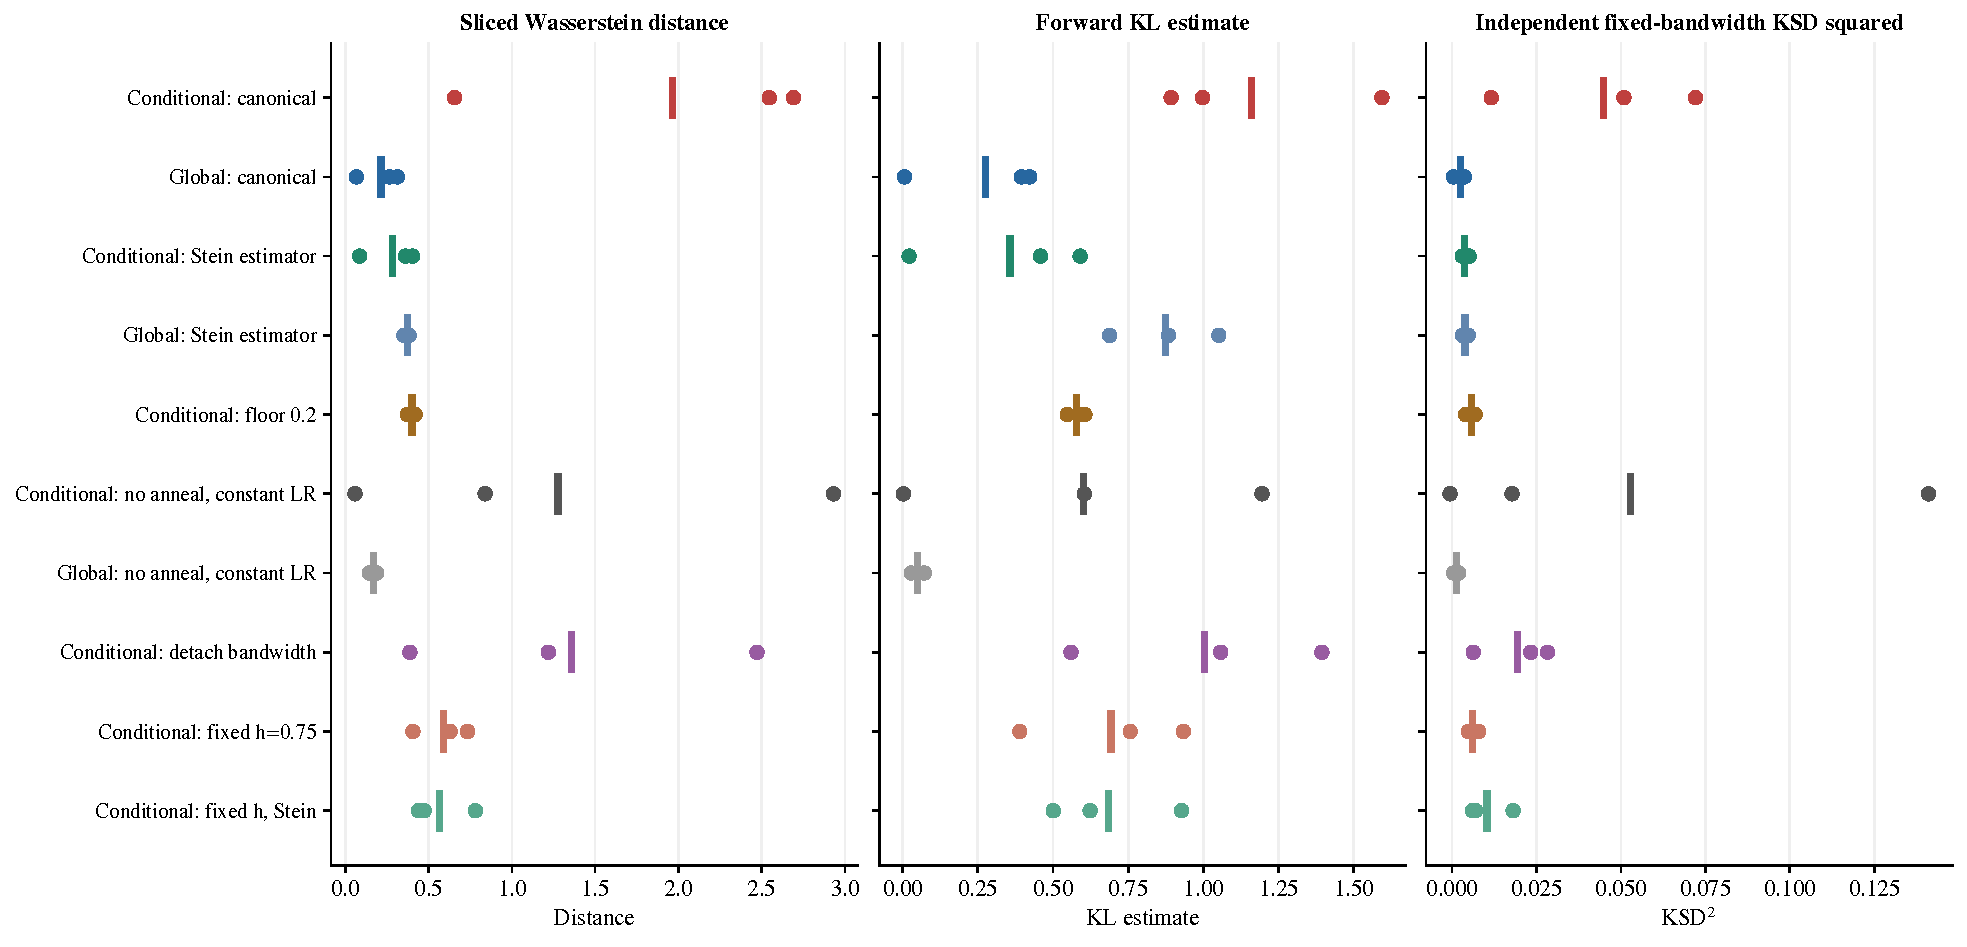
\includegraphics[width=\linewidth,height=.76\textheight,keepaspectratio]{figures/confirmation.pdf}
\caption{Matched comparisons after 50,000 updates. Dots are independently trained seeds 42--44; vertical strokes mark means. Initial mean weights, variance values, and training noise are paired. Forward KL uses the largest evaluated latent mixture; held-out KSD uses an independent fixed bandwidth of 0.75.}
\end{figure}
\clearpage
\begin{figure}[!ht]
\centering
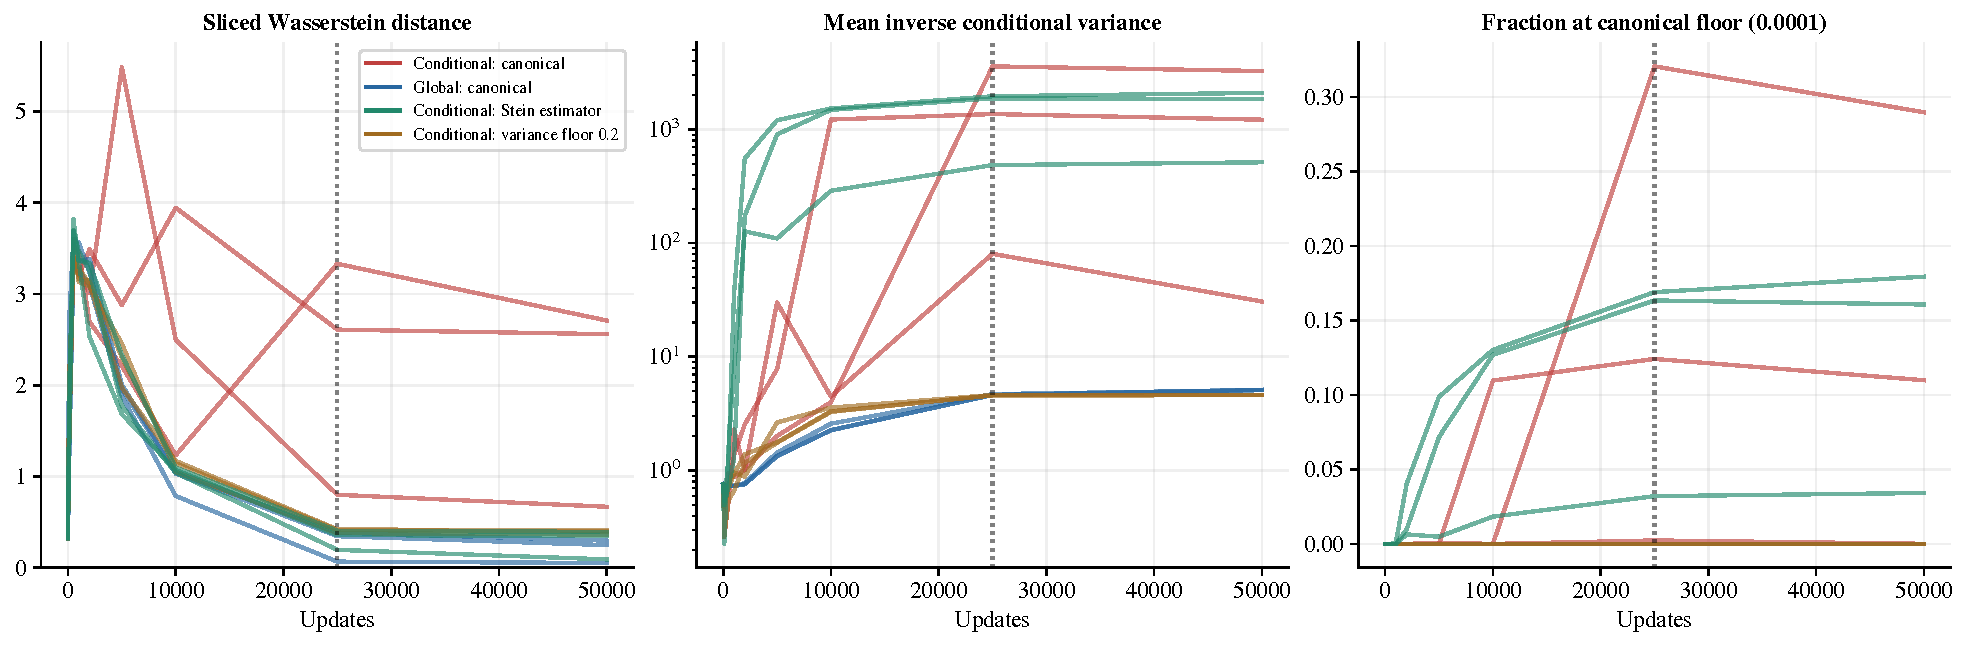
\includegraphics[width=\linewidth,height=.76\textheight,keepaspectratio]{figures/trajectories.pdf}
\caption{Accuracy and the small-variance tail across three trajectories per procedure. The dotted line marks completion of target annealing at update 25,000. Floor occupancy uses the common threshold 0.00010001; diagnostic draws preserve training RNG.}
\end{figure}
\clearpage
\begin{figure}[!ht]
\centering
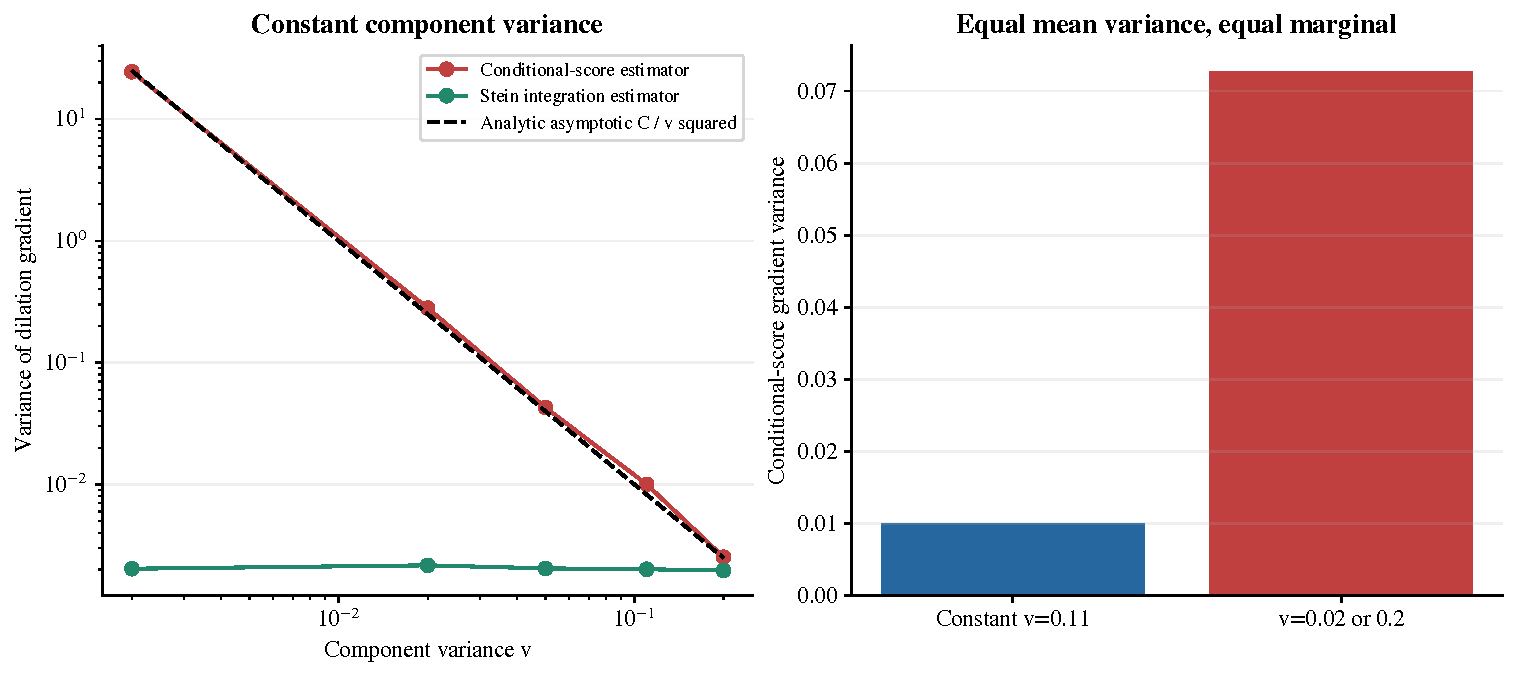
\includegraphics[width=\linewidth,height=.76\textheight,keepaspectratio]{figures/exact_marginal_noise.pdf}
\caption{Representation noise at exactly equal marginal distributions. Each measurement uses 256 independent repetitions and two batches of 128 at fixed bandwidth 0.75. The dashed curve is the analytic small-variance prediction, with no fitted coefficient. The right panel holds both the marginal and mean component variance 0.11 fixed.}
\end{figure}
\clearpage
\begin{figure}[!ht]
\centering
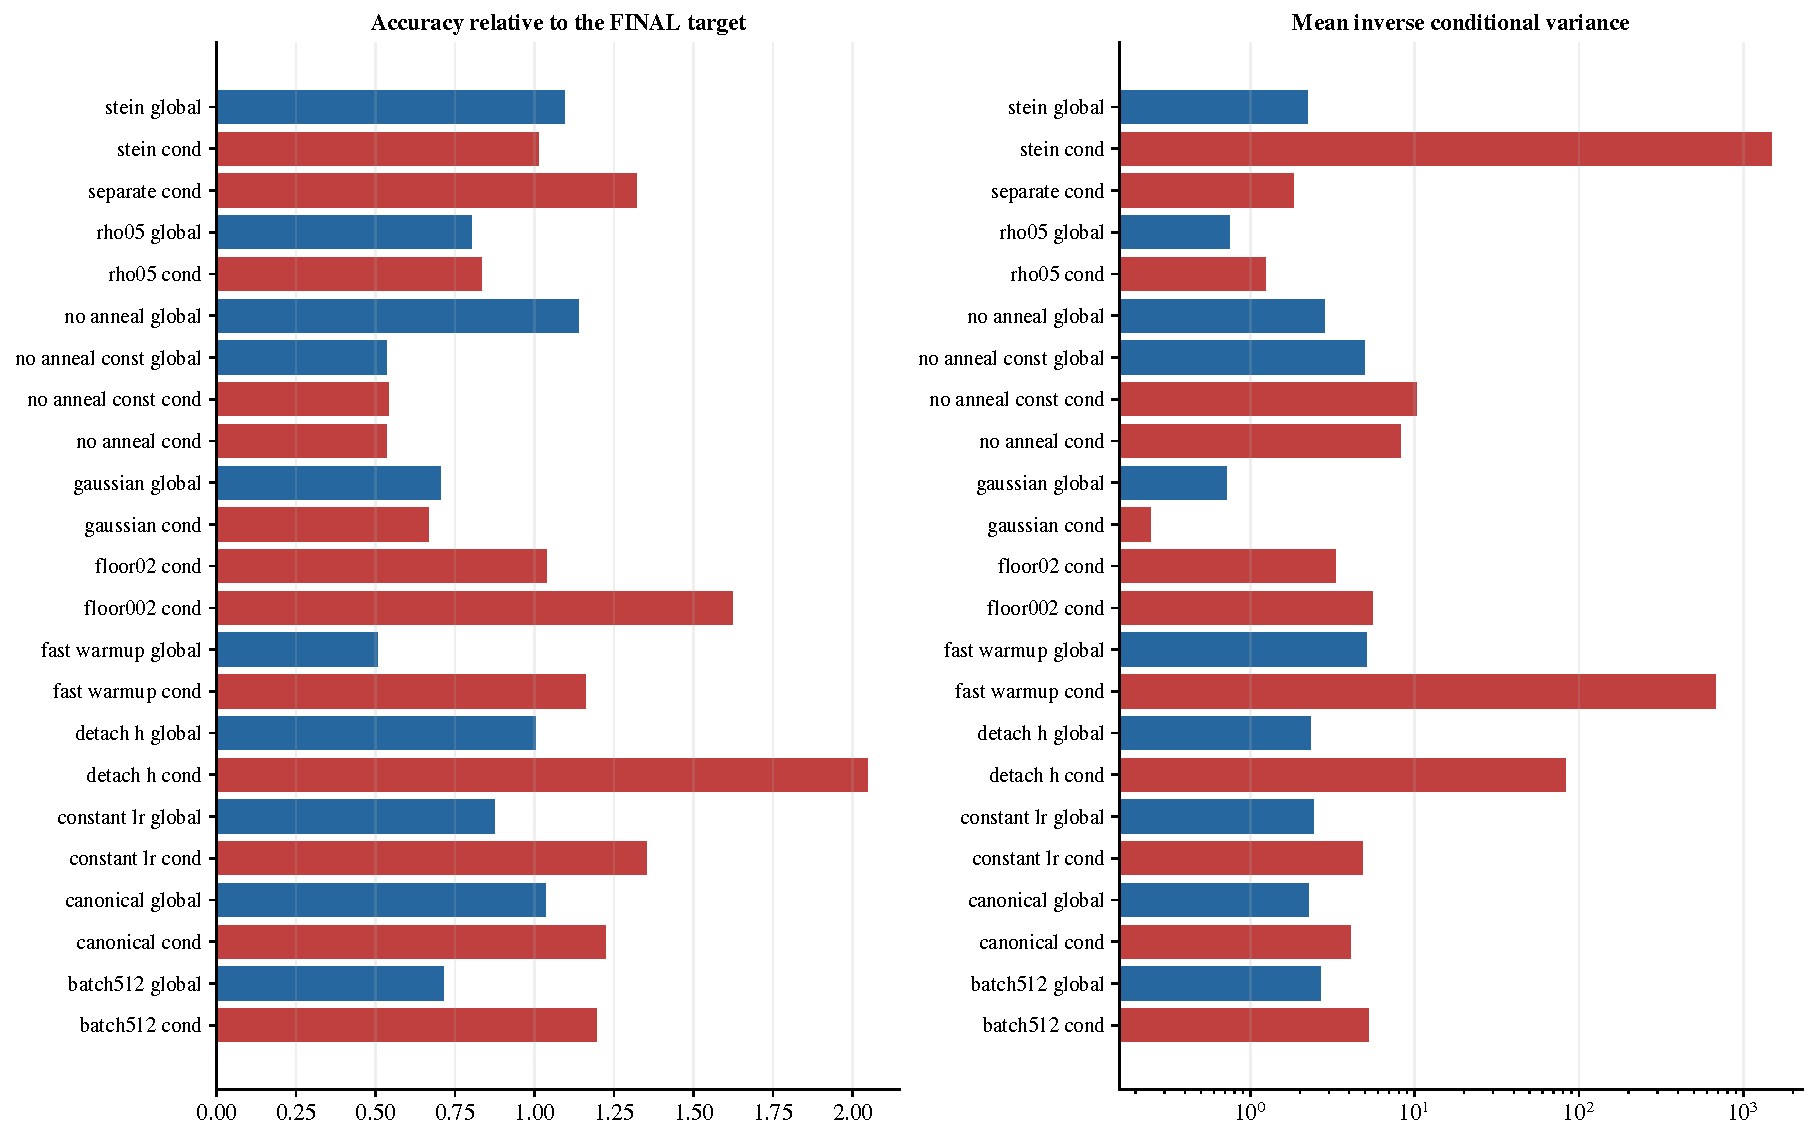
\includegraphics[width=\linewidth,height=.76\textheight,keepaspectratio]{figures/screening.pdf}
\caption{All 23 screening outcomes at 10,000 updates, seed 42. Blue denotes global variance; red denotes conditional variance. Annealed runs still have a score multiplier of 0.46 unless warmup is shortened. Distances are measured against the final target and do not establish final-target convergence.}
\end{figure}
\clearpage
\begin{figure}[!ht]
\centering
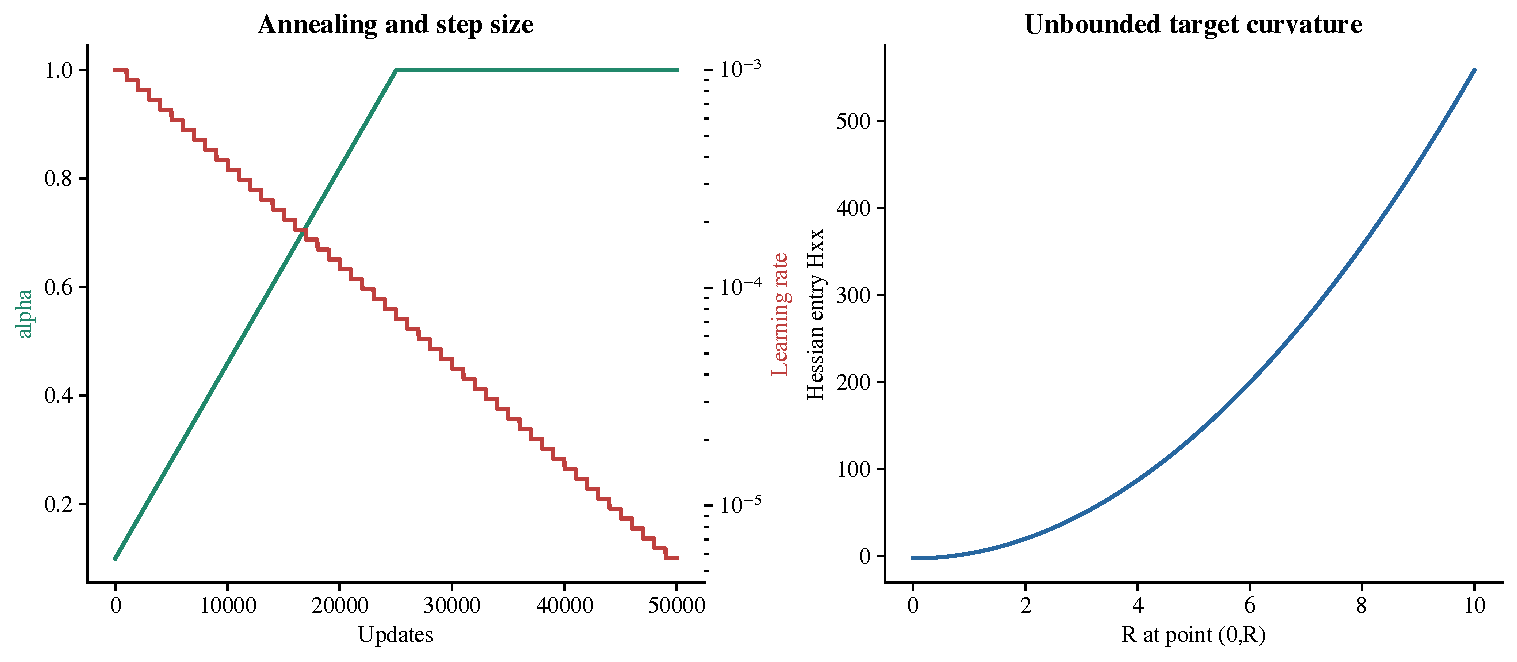
\includegraphics[width=\linewidth,height=.76\textheight,keepaspectratio]{figures/geometry_and_schedule.pdf}
\caption{Target path, learning-rate decay, and target curvature. The score multiplier reaches one after the learning rate has fallen to approximately 0.0000718. The diverging Hessian entry violates the global bounded-Hessian assumption for both variational families; this fact alone does not explain their ordering.}
\end{figure}
\clearpage
\begin{figure}[!ht]
\centering
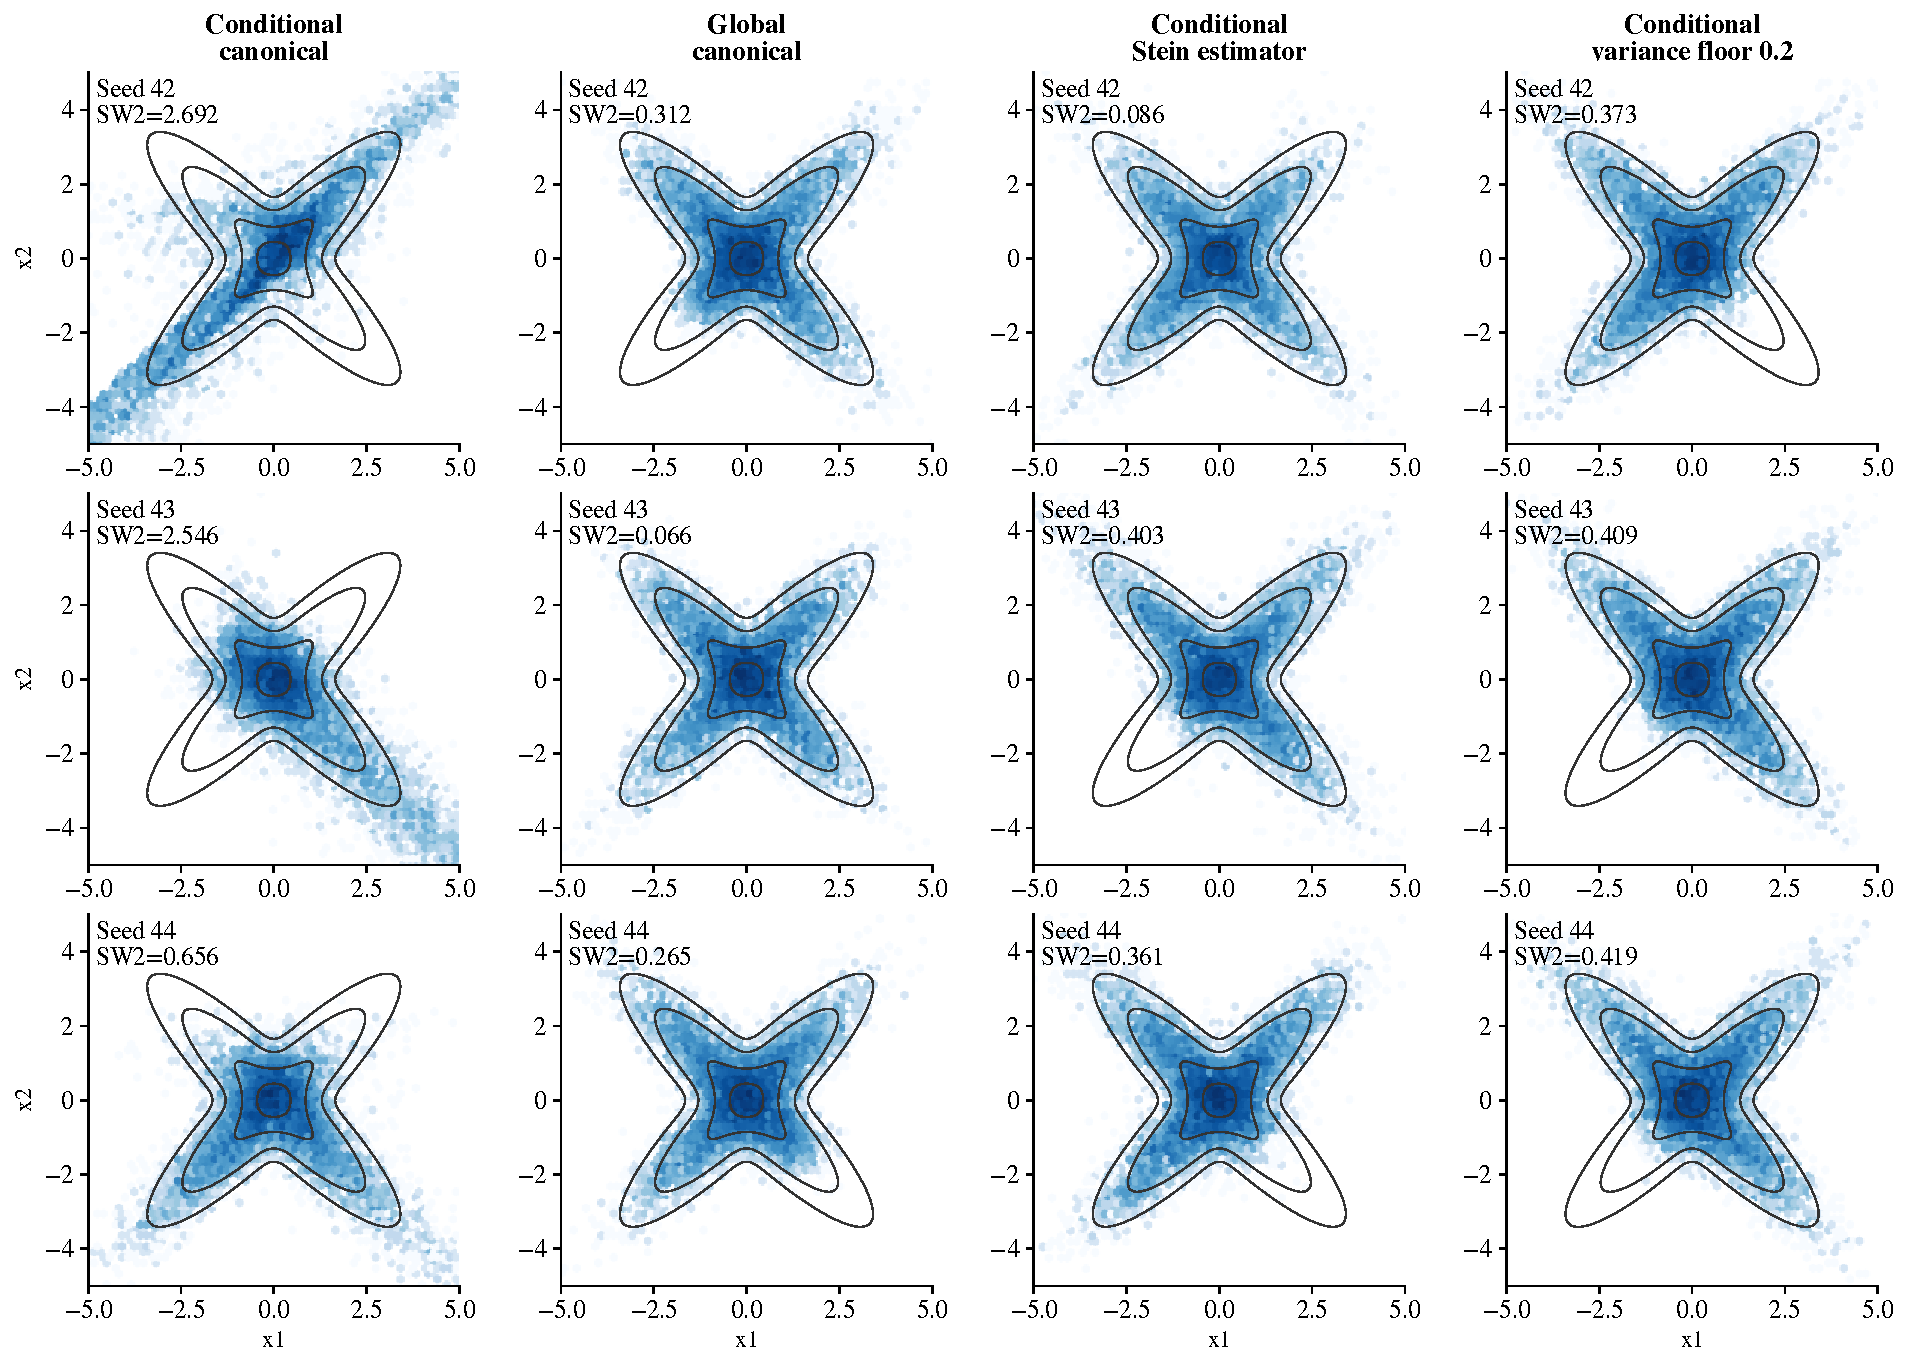
\includegraphics[width=\linewidth,height=.76\textheight,keepaspectratio]{figures/final_samples.pdf}
\caption{Final samples for seeds 42--44, with exact target contours and a common viewing window. All samples contribute to numerical metrics, including tails outside the plot. The separate sample pages in the companion booklet provide larger panels for each seed.}
\end{figure}
\end{landscape}

\begin{thebibliography}{9}
\bibitem{cheng} Z. Cheng, L. Yu, T. Xie, S. Zhang and C. Zhang (2024).
Kernel Semi-Implicit Variational Inference. ICML, PMLR 235:8248--8269.
\url{https://proceedings.mlr.press/v235/cheng24l.html}.
\bibitem{yu} L. Yu, Z. Cheng, S. Zhang and C. Zhang (2026).
A Kernel Approach for Semi-implicit Variational Inference.
\url{https://arxiv.org/abs/2601.12023}. Appendix A.4 documents global
variance in the experiments; Appendix C.1 gives toy-model settings.
\bibitem{korba} A. Korba, P.-C. Aubin-Frankowski, S. Majewski and P. Ablin
(2021). Kernel Stein Discrepancy Descent. ICML, PMLR 139:5719--5730.
\url{https://proceedings.mlr.press/v139/korba21a.html}.
\bibitem{code} Original KSIVI implementation:
\url{https://github.com/longinYu/KSIVI}.
\end{thebibliography}
\end{document}
